\tikzstyle{nodus}=[circle,draw=black,minimum size=1.5 cm,text width=1.5cm,align=center]
\def\dis{1.5}
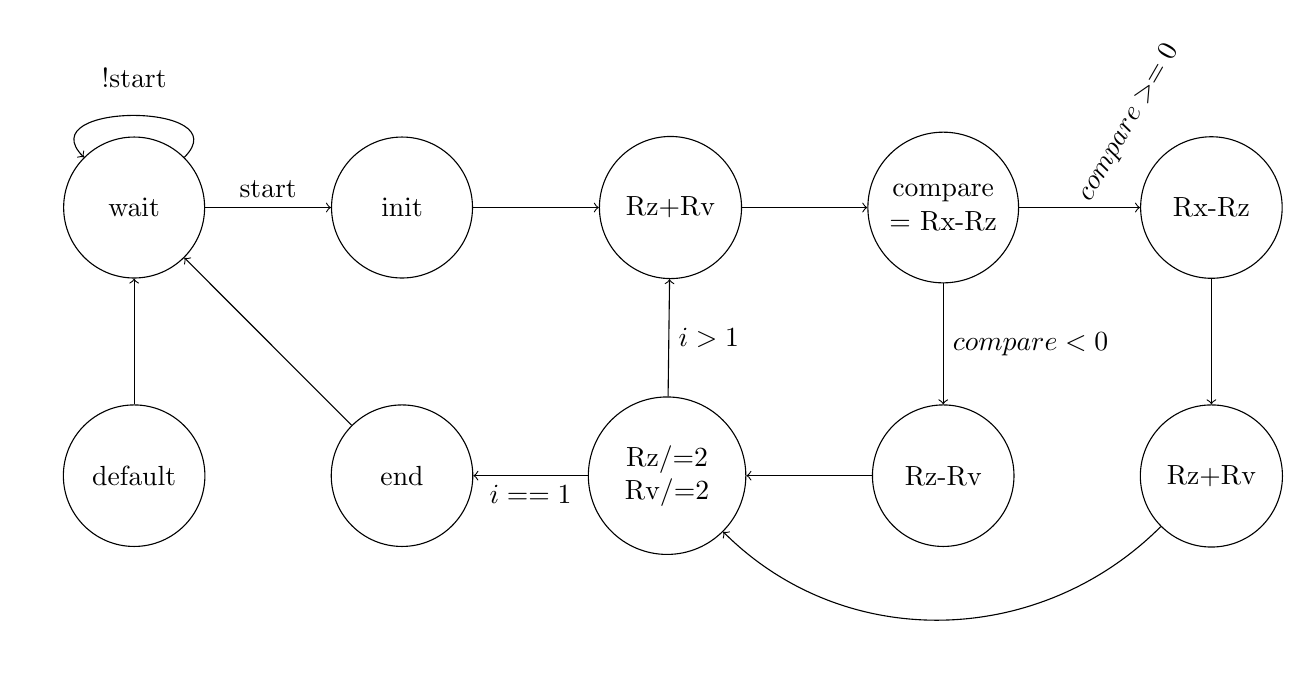
\begin{tikzpicture}
\node [nodus] (wait)	[label={[label distance=0.5cm]90:!start}]  at (0,0) {wait};
\node [nodus] (init) 	[right of = wait,right = \dis cm] {init};
\node [nodus] (end) 	[below of = init,below= \dis cm] {end};
\node [nodus] (default) [below of = wait,below= \dis cm] {default};
\node [nodus] (iter1) [right of = init, right= \dis cm] {Rz+Rv};
\node [nodus] (iter2) [right of = iter1, right= \dis cm] {compare = Rx-Rz};

\node [nodus] (iter3_bis) [below of = iter2,below= \dis cm] {Rz-Rv};

\node [nodus] (iter3) [right of = iter2, right= \dis cm] {Rx-Rz};
\node [nodus] (iter4) [below of = iter3, below= \dis cm] {Rz+Rv};
\node [nodus] (iter5) [left of = iter3_bis, left= \dis cm] {Rz/=2 Rv/=2};


\draw [->] (wait) edge node [midway,above]{start}  (init);
\draw [->] (init)   edge (iter1);
\draw [->] (iter1) edge (iter2);
\draw [->] (iter2) edge node [rotate=60,midway,right]{$compare >= 0$}(iter3);
\draw [->] (iter3) edge  (iter4);
\draw [->] (iter4) to [in=-45,out=-135] (iter5);
%%%%%
\draw [->] (iter2) edge node [midway, right]{$compare < 0$}(iter3_bis);
\draw [->] (iter3_bis) edge (iter5);
%%%%%
\draw [->] (iter5) edge node [midway,below] {$i==1$}(end);
\draw [->] (iter5) edge node [midway,right] {$i > 1$} (iter1);

%\draw [->] (iter)  edge node [midway,above]{i==n}  (end);
\draw [->] (end) edge (wait);
\draw [->] (default) edge (wait);

\draw [->](wait)  to[distance = 1 cm ,out=45,in=135] (wait);


\end{tikzpicture}